%===============================================================================
% LaTeX sjabloon voor de bachelorproef toegepaste informatica aan HOGENT
% Meer info op https://github.com/HoGentTIN/latex-hogent-report
%===============================================================================

\documentclass[dutch,dit,thesis]{hogentreport}

% TODO:
% - If necessary, replace the option `dit`' with your own department!
%   Valid entries are dbo, dbt, dgz, dit, dlo, dog, dsa, soa
% - If you write your thesis in English (remark: only possible after getting
%   explicit approval!), remove the option "dutch," or replace with "english".

\usepackage{lipsum} % For blind text, can be removed after adding actual content
\usepackage[absolute,showboxes]{textpos}

\setlength{\TPHorizModule}{1mm}
\setlength{\TPVertModule}{1mm}
\setlength{\parindent}{0mm}

%% Pictures to include in the text can be put in the graphics/ folder
\graphicspath{{../graphics/}}

%% For source code highlighting, requires pygments to be installed
%% Compile with the -shell-escape flag!
%% \usepackage[chapter]{minted}
%% If you compile with the make_thesis.{bat,sh} script, use the following
%% import instead:
\usepackage[chapter,outputdir=../output]{minted}
\usemintedstyle{solarized-light}

%% Formatting for minted environments.
\setminted{%
    autogobble,
    frame=lines,
    breaklines,
    linenos,
    tabsize=4
}

%% Ensure the list of listings is in the table of contents
\renewcommand\listoflistingscaption{%
    \IfLanguageName{dutch}{Lijst van codefragmenten}{List of listings}
}
\renewcommand\listingscaption{%
    \IfLanguageName{dutch}{Codefragment}{Listing}
}
\renewcommand*\listoflistings{%
    \cleardoublepage\phantomsection\addcontentsline{toc}{chapter}{\listoflistingscaption}%
    \listof{listing}{\listoflistingscaption}%
}

% Other packages not already included can be imported here

%%---------- Document metadata -------------------------------------------------
% TODO: Replace this with your own information
\author{Vandenbroucke Jasper}
\supervisor{Mevr. S. Vandermeersch}
\cosupervisor{Dhr. C. Cokelaere}
\title{Optimalisatie van webapplicaties met behulp van microservices-architectuur bij stagebedrijf Fabrimode: een onderzoek naar schaalbaarheid en complexiteit.}
\academicyear{\advance\year by -1 \the\year--\advance\year by 1 \the\year}
\examperiod{1}
\degreesought{\IfLanguageName{dutch}{Professionele bachelor in de toegepaste informatica}{Bachelor of applied computer science}}
\partialthesis{false} %% To display 'in partial fulfilment'
%\institution{Internshipcompany BVBA.}

%% Add global exceptions to the hyphenation here
\hyphenation{back-slash}

%% The bibliography (style and settings are  found in hogentthesis.cls)
\addbibresource{bachproef.bib}            %% Bibliography file
\addbibresource{../voorstel/voorstel.bib} %% Bibliography research proposal
\defbibheading{bibempty}{}

%% Prevent empty pages for right-handed chapter starts in twoside mode
\renewcommand{\cleardoublepage}{\clearpage}

\renewcommand{\arraystretch}{1.2}

%% Content starts here.
\begin{document}

%---------- Front matter -------------------------------------------------------

\frontmatter

\hypersetup{pageanchor=false} %% Disable page numbering references
%% Render a Dutch outer title page if the main language is English
\IfLanguageName{english}{%
    %% If necessary, information can be changed here
    \degreesought{Professionele Bachelor toegepaste informatica}%
    \begin{otherlanguage}{dutch}%
       \maketitle%
    \end{otherlanguage}%
}{}

%% Generates title page content
\maketitle
\hypersetup{pageanchor=true}

%%=============================================================================
%% Voorwoord
%%=============================================================================

\chapter*{\IfLanguageName{dutch}{Woord vooraf}{Preface}}%
\label{ch:voorwoord}

%% TODO:
%% Het voorwoord is het enige deel van de bachelorproef waar je vanuit je
%% eigen standpunt (``ik-vorm'') mag schrijven. Je kan hier bv. motiveren
%% waarom jij het onderwerp wil bespreken.
%% Vergeet ook niet te bedanken wie je geholpen/gesteund/... heeft

Met trots presenteer ik u mijn bachelorproef, "Optimalisatie van webapplicaties met behulp van microservices-architectuur bij stagebedrijf Fabrimode: een onderzoek naar schaalbaarheid en complexiteit.", geschreven ter afronding van mijn opleiding Bachelor in de Toegepaste Informatica aan de Hogeschool Gent. Deze bachelorproef is het sluitstuk van een intensieve, maar vooral enorm verrijkende periode van drie jaar. Toen ik aan deze studie begon, beschikte ik over nagenoeg geen programmeerkennis. Vandaag de dag, aan het einde van deze opleiding, ben ik bijzonder trots op de vaardigheden die ik heb verworven. Deze transformatie van complete beginner tot een programmeur met een solide fundament in softwareontwikkeling was een belangrijke motivatie voor de keuze van dit bachelorproefonderwerp.\newline

Tijdens mijn opzoekwerk besefte ik dat de projecten waarmee ik tot dan toe in aanraking was gekomen voornamelijk gebaseerd waren op een monolithische architectuur. Naarmate ik meer leerde over modernere architecturen zoals microservices, begon ik me af te vragen of de traditionele monoliet wel de meest geschikte keuze is voor grootschalige applicaties. Microservices worden vaak genoemd in de context van schaalbare systemen, maar brengen ook nieuwe uitdagingen met zich mee. Hierdoor wilde ik beter begrijpen hoe beide architecturen zich in de praktijk van elkaar onderscheiden. Zo kwam ik op het idee om hun prestaties en codecomplexiteit tegenover elkaar te plaatsen in een concrete uitwerking.\newline

Deze bachelorproef had ik niet kunnen realiseren zonder de steun van enkele belangrijke personen. In het bijzonder wil ik mijn promotor, mevrouw Sonia Vandermeersch, bedanken voor haar waardevolle begeleiding en feedback gedurende de uitwerking van deze bachelorproef. Ook mijn co-promotor, de heer Chris Cokelaere, wil ik hartelijk bedanken voor zijn ondersteuning en betrokkenheid, zowel bij de bachelorproef als bij de stage.\newline

Tot slot dank ik u, beste lezer, om interesse te tonen en de tijd te nemen deze bachelorproef door te nemen.\newline

Vandenbroucke Jasper
%%=============================================================================
%% Samenvatting
%%=============================================================================

% TODO: De "abstract" of samenvatting is een kernachtige (~ 1 blz. voor een
% thesis) synthese van het document.
%
% Een goede abstract biedt een kernachtig antwoord op volgende vragen:
%
% 1. Waarover gaat de bachelorproef?
% 2. Waarom heb je er over geschreven?
% 3. Hoe heb je het onderzoek uitgevoerd?
% 4. Wat waren de resultaten? Wat blijkt uit je onderzoek?
% 5. Wat betekenen je resultaten? Wat is de relevantie voor het werkveld ?
%
% Daarom bestaat een abstract uit volgende componenten:
%
% - inleiding + kaderen thema
% - probleemstelling
% - (centrale) onderzoeksvraag
% - onderzoeksdoelstelling
% - methodologie
% - resultaten (beperk tot de belangrijkste, relevant voor de onderzoeksvraag)
% - conclusies, aanbevelingen, beperkingen
%
% LET OP! Een samenvatting is GEEN voorwoord!

%%---------- Nederlandse samenvatting -----------------------------------------
%
% TODO: Als je je bachelorproef in het Engels schrijft, moet je eerst een
% Nederlandse samenvatting invoegen. Haal daarvoor onderstaande code uit
% commentaar.
% Wie zijn bachelorproef in het Nederlands schrijft, kan dit negeren, de inhoud
% wordt niet in het document ingevoegd.

%\IfLanguageName{english}{%
%\selectlanguage{dutch}
%\chapter*{Samenvatting}
%\lipsum[1-4]
%\selectlanguage{english}
%}{}

%%---------- Samenvatting -----------------------------------------------------
% De samenvatting in de hoofdtaal van het document

\chapter{Samenvatting}

De impact van een microservices-architectuur op de schaalbaarheid en complexiteit van webapplicaties staat centraal in deze bachelorproef. Het stagebedrijf Fabrimode wil weten of een overstap naar microservices de prestaties van een webapplicatie kunnen verbeteren. In de hedendaagse softwareontwikkeling, waarin schaalbaarheid en onderhoudbaarheid van cruciaal belang zijn, biedt de microservices-architectuur een alternatief door applicaties op te splitsen in onafhankelijke services. Daarom luidt de onderzoeksvraag als volgt: "Welke impact heeft een microservices\--architectuur op de schaalbaarheid en ontwikkelingscomplexiteit van een webapplicatie?".\newline

De monolithische architectuur ondervindt vaak schaalbaarheidsproblemen bij groei, terwijl microservices een mogelijke oplossing bieden voor dit probleem, maar mogelijks de ontwikkelingscomplexiteit verhogen. Het doel van deze bachelorproef is om na te gaan of microservices een optimalisatie bieden op het gebied van schaalbaarheid en complexiteit. Dit zal bekeken worden aan de hand van een proof-of-concept (PoC), die in hoofdstuk \ref{ch:methodologie} verder wordt toegelicht.\newline

De methodologie die zal toegepast worden bestaat in eerste instantie uit een literatuurstudie, waarin de verschillen tussen beide architecturen nader bekeken zullen worden. Volgend op de literatuurstudie is het ontwikkelen van een proof-of-concept (PoC) met twee versies van een e-commerce webapplicatie (monolithisch en microservices). Beide zullen voornamelijk ontwikkeld worden in C\# met .NET 8. Eén service van de mircoservices-applicatie zal met Node.js en Express ontwikkeld worden, om de flexibiliteit binnen een microservices-architectuur te demonstreren. Daarnaast zal voor het implementeren en beheren van microservices gebruik gemaakt worden van Docker en Kubernetes samen met RabbitMQ als communicatie tool. Tot slot zullen na het uitwerken van de PoC de schaalbaarheid en complexiteit getest en geanalyseerd worden met respectievelijk Apache JMeter en SonarQube als tools.\newline


%---------- Inhoud, lijst figuren, ... -----------------------------------------

\tableofcontents

% In a list of figures, the complete caption will be included. To prevent this,
% ALWAYS add a short description in the caption!
%
%  \caption[short description]{elaborate description}
%
% If you do, only the short description will be used in the list of figures

\listoffigures

% If you included tables and/or source code listings, uncomment the appropriate
% lines.
\listoftables

\listoflistings

% Als je een lijst van afkortingen of termen wil toevoegen, dan hoort die
% hier thuis. Gebruik bijvoorbeeld de ``glossaries'' package.
% https://www.overleaf.com/learn/latex/Glossaries

%---------- Kern ---------------------------------------------------------------

\mainmatter{}

% De eerste hoofdstukken van een bachelorproef zijn meestal een inleiding op
% het onderwerp, literatuurstudie en verantwoording methodologie.
% Aarzel niet om een meer beschrijvende titel aan deze hoofdstukken te geven of
% om bijvoorbeeld de inleiding en/of stand van zaken over meerdere hoofdstukken
% te verspreiden!

%%=============================================================================
%% Inleiding
%%=============================================================================

\chapter{\IfLanguageName{dutch}{Inleiding}{Introduction}}%
\label{ch:inleiding}

\section{Context en achtergrond}

In de moderne softwareontwikkeling wordt steeds vaker gezocht naar schaalbare en onderhoudbare architecturen om de groeiende complexiteit van webapplicaties aan te kunnen. Traditioneel zijn heel wat applicaties ontwikkeld volgens een monolithische architectuur, waarbij alle functionaliteiten binnen één en dezelfde codebase beheert worden. In de beginfase van een applicatie/project zijn voordelen heeft, zoals eenvoudige ontwikkeling en implementatie, kan het bij groeiende applicaties tot schaalbaarheid- en onderhoudbaarheidsproblemen leiden.

Om deze problemen te voorkomen, wordt steeds vaker overgestapt naar een microservices-architectuur. Deze architectuurstijl verdeelt een applicatie in meerdere kleine, onafhankelijke services, die elk een specifieke bedrijfsfunctionaliteit op zich nemen, zoals productenbeheer, bestellingen, gebruikers-/klantenbeheer enz. Deze aparte services communiceren met elkaar via API's (zoals REST of gRPC). Het grootste voordeel bij microservices is op het gebied van schaalbaarheid, flexibiliteit en onderhoudbaarheid, maar als kanttekening brengen ze een extra uitdaging met zich mee, zoals dataconsistentie en orkestratie.

Bij het stagebedrijf Fabrimode, dat actief is binnen de mode-industrie, is er interesse in het onderzoeken van de opties van microservices. Daarom zal in dit onderzoek de focus liggen op de potentiële voordelen van een overgang naar microservices. Het hoofddoel van deze bachelorproef is om inzicht te krijgen in de mogelijkheden van deze technologie voor Fabrimode.

%De inleiding moet de lezer net genoeg informatie verschaffen om het onderwerp te begrijpen en in te zien waarom de onderzoeksvraag de moeite waard is om te onderzoeken. In de inleiding ga je literatuurverwijzingen beperken, zodat de tekst vlot leesbaar blijft. Je kan de inleiding verder onderverdelen in secties als dit de tekst verduidelijkt. Zaken die aan bod kunnen komen in de inleiding~\autocite{Pollefliet2011}:

%\begin{itemize}
%  \item context, achtergrond
%  \item afbakenen van het onderwerp
%  \item verantwoording van het onderwerp, methodologie
%  \item probleemstelling
%  \item onderzoeksdoelstelling
%  \item onderzoeksvraag
%  \item \ldots
%\end{itemize}

%\section{\IfLanguageName{dutch}{Probleemstelling}{Problem Statement}}%
%\label{sec:probleemstelling}

%Uit je probleemstelling moet duidelijk zijn dat je onderzoek een meerwaarde heeft voor een concrete doelgroep. De doelgroep moet goed gedefinieerd en afgelijnd zijn. Doelgroepen als ``bedrijven,'' ``KMO's'', systeembeheerders, enz.~zijn nog te vaag. Als je een lijstje kan maken van de personen/organisaties die een meerwaarde zullen vinden in deze bachelorproef (dit is eigenlijk je steekproefkader), dan is dat een indicatie dat de doelgroep goed gedefinieerd is. Dit kan een enkel bedrijf zijn of zelfs één persoon (je co-promotor/opdrachtgever).

%\section{\IfLanguageName{dutch}{Onderzoeksvraag}{Research question}}%
%\label{sec:onderzoeksvraag}

%Wees zo concreet mogelijk bij het formuleren van je onderzoeksvraag. Een onderzoeksvraag is trouwens iets waar nog niemand op dit moment een antwoord heeft (voor zover je kan nagaan). Het opzoeken van bestaande informatie (bv. ``welke tools bestaan er voor deze toepassing?'') is dus geen onderzoeksvraag. Je kan de onderzoeksvraag verder specifiëren in deelvragen. Bv.~als je onderzoek gaat over performantiemetingen, dan 

%\section{\IfLanguageName{dutch}{Onderzoeksdoelstelling}{Research objective}}%
%\label{sec:onderzoeksdoelstelling}

%Wat is het beoogde resultaat van je bachelorproef? Wat zijn de criteria voor succes? Beschrijf die zo concreet mogelijk. Gaat het bv.\ om een proof-of-concept, een prototype, een verslag met aanbevelingen, een vergelijkende studie, enz.

%\section{\IfLanguageName{dutch}{Opzet van deze bachelorproef}{Structure of this bachelor thesis}}%
%\label{sec:opzet-bachelorproef}

% Het is gebruikelijk aan het einde van de inleiding een overzicht te
% geven van de opbouw van de rest van de tekst. Deze sectie bevat al een aanzet
% die je kan aanvullen/aanpassen in functie van je eigen tekst.

%De rest van deze bachelorproef is als volgt opgebouwd:

%In Hoofdstuk~\ref{ch:stand-van-zaken} wordt een overzicht gegeven van de stand van zaken binnen het onderzoeksdomein, op basis van een literatuurstudie.

%In Hoofdstuk~\ref{ch:methodologie} wordt de methodologie toegelicht en worden de gebruikte onderzoekstechnieken besproken om een antwoord te kunnen formuleren op de onderzoeksvragen.

%% TODO: Vul hier aan voor je eigen hoofstukken, één of twee zinnen per hoofdstuk

%In Hoofdstuk~\ref{ch:conclusie}, tenslotte, wordt de conclusie gegeven en een antwoord geformuleerd op de onderzoeksvragen. Daarbij wordt ook een aanzet gegeven voor toekomstig onderzoek binnen dit domein.
\chapter{\IfLanguageName{dutch}{Stand van zaken}{State of the art}}%
\label{ch:stand-van-zaken}

In dit hoofdstuk van de bachelorproef zullen we dieper ingaan op het concept van een microservices-architectuur. Dit zal gebeuren aan de hand van een relevante literatuurstudie. Allereerst zal uitgelegd worden wat een monolithische architectuur is en wat typerend is aan deze stijl van software ontwikkeling. Daarna wordt uitgelegd wat een microservices-architectuur is en hoe deze architectuur verschilt van de klassieke, monolithische aanpak. Vervolgens worden enkele relevante termen uitgereider behandelt die de werking en structuur van microservices definiëren. Tot slot zal er gekeken worden naar de nodige tools om microservices te ontwikkelen en beheren.

\section{Wat is een monolithische architectuur?}

\section{Wat is een microservices-architectuur?}

% Tip: Begin elk hoofdstuk met een paragraaf inleiding die beschrijft hoe
% dit hoofdstuk past binnen het geheel van de bachelorproef. Geef in het
% bijzonder aan wat de link is met het vorige en volgende hoofdstuk.

% Pas na deze inleidende paragraaf komt de eerste sectiehoofding.

%Dit hoofdstuk bevat je literatuurstudie. De inhoud gaat verder op de inleiding, maar zal het onderwerp van de bachelorproef *diepgaand* uitspitten. De %bedoeling is dat de lezer na lezing van dit hoofdstuk helemaal op de hoogte is van de huidige stand van zaken (state-of-the-art) in het %onderzoeksdomein. Iemand die niet vertrouwd is met het onderwerp, weet nu voldoende om de rest van het verhaal te kunnen volgen, zonder dat die er nog %andere informatie moet over opzoeken \autocite{Pollefliet2011}.

%Je verwijst bij elke bewering die je doet, vakterm die je introduceert, enz.\ naar je bronnen. In \LaTeX{} kan dat met het commando %\texttt{$\backslash${textcite\{\}}} of \texttt{$\backslash${autocite\{\}}}. Als argument van het commando geef je de ``sleutel'' van een ``record'' in %een bibliografische databank in het Bib\LaTeX{}-formaat (een tekstbestand). Als je expliciet naar de auteur verwijst in de zin (narratieve %referentie), gebruik je \texttt{$\backslash${}textcite\{\}}. Soms is de auteursnaam niet expliciet een onderdeel van de zin, dan gebruik je %\texttt{$\backslash${}autocite\{\}} (referentie tussen haakjes). Dit gebruik je bv.~bij een citaat, of om in het bijschrift van een overgenomen %afbeelding, broncode, tabel, enz. te verwijzen naar de bron. In de volgende paragraaf een voorbeeld van elk.

%\textcite{Knuth1998} schreef een van de standaardwerken over sorteer- en zoekalgoritmen. Experten zijn het erover eens dat cloud computing een %interessante opportuniteit vormen, zowel voor gebruikers als voor dienstverleners op vlak van informatietechnologie~\autocite{Creeger2009}.

%Let er ook op: het \texttt{cite}-commando voor de punt, dus binnen de zin. Je verwijst meteen naar een bron in de eerste zin die erop gebaseerd is, %dus niet pas op het einde van een paragraaf.

%\begin{figure}
%  \centering
%  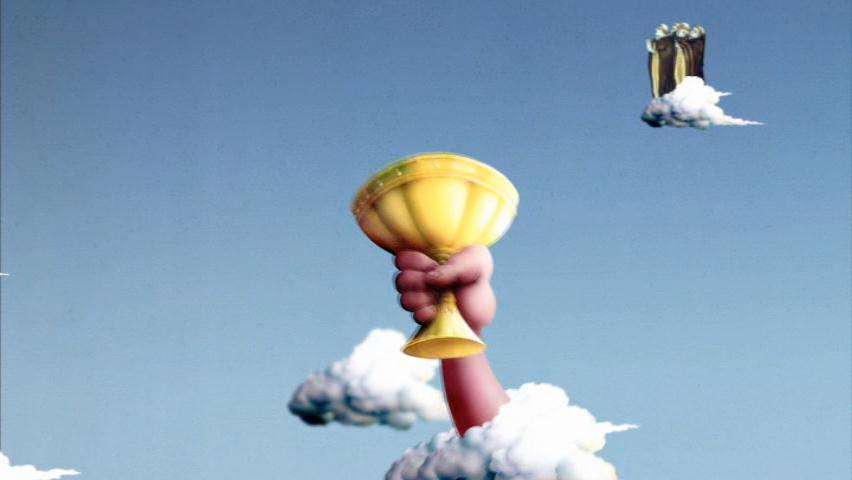
\includegraphics[width=0.8\textwidth]{grail.jpg}
%  \caption[Voorbeeld figuur.]{\label{fig:grail}Voorbeeld van invoegen van een figuur. Zorg altijd voor een uitgebreid bijschrift dat de figuur %volledig beschrijft zonder in de tekst te moeten gaan zoeken. Vergeet ook je bronvermelding niet!}
%\end{figure}

%\begin{listing}
%  \begin{minted}{python}
%    import pandas as pd
%    import seaborn as sns
%
%    penguins = sns.load_dataset('penguins')
%    sns.relplot(data=penguins, x="flipper_length_mm", y="bill_length_mm", hue="species")
%  \end{minted}
%  \caption[Voorbeeld codefragment]{Voorbeeld van het invoegen van een codefragment.}
%\end{listing}

%\lipsum[7-20]

%\begin{table}
%  \centering
%  \begin{tabular}{lcr}
%    \toprule
%    \textbf{Kolom 1} & \textbf{Kolom 2} & \textbf{Kolom 3} \\
%    $\alpha$         & $\beta$          & $\gamma$         \\
%    \midrule
%    A                & 10.230           & a                \\
%    B                & 45.678           & b                \\
%    C                & 99.987           & c                \\
%    \bottomrule
%  \end{tabular}
%  \caption[Voorbeeld tabel]{\label{tab:example}Voorbeeld van een tabel.}
%\end{table}


%%=============================================================================
%% Methodologie
%%=============================================================================

\chapter{\IfLanguageName{dutch}{Methodologie}{Methodology}}%
\label{ch:methodologie}

%% TODO: In dit hoofstuk geef je een korte toelichting over hoe je te werk bent
%% gegaan. Verdeel je onderzoek in grote fasen, en licht in elke fase toe wat
%% de doelstelling was, welke deliverables daar uit gekomen zijn, en welke
%% onderzoeksmethoden je daarbij toegepast hebt. Verantwoord waarom je
%% op deze manier te werk gegaan bent.
%% 
%% Voorbeelden van zulke fasen zijn: literatuurstudie, opstellen van een
%% requirements-analyse, opstellen long-list (bij vergelijkende studie),
%% selectie van geschikte tools (bij vergelijkende studie, "short-list"),
%% opzetten testopstelling/PoC, uitvoeren testen en verzamelen
%% van resultaten, analyse van resultaten, ...
%%
%% !!!!! LET OP !!!!!
%%
%% Het is uitdrukkelijk NIET de bedoeling dat je het grootste deel van de corpus
%% van je bachelorproef in dit hoofstuk verwerkt! Dit hoofdstuk is eerder een
%% kort overzicht van je plan van aanpak.
%%
%% Maak voor elke fase (behalve het literatuuronderzoek) een NIEUW HOOFDSTUK aan
%% en geef het een gepaste titel.

\lipsum[21-25]



% Voeg hier je eigen hoofdstukken toe die de ``corpus'' van je bachelorproef
% vormen. De structuur en titels hangen af van je eigen onderzoek. Je kan bv.
% elke fase in je onderzoek in een apart hoofdstuk bespreken.

%\input{...}
%\input{...}
%...

%%=============================================================================
%% Conclusie
%%=============================================================================

\chapter{Conclusie}%
\label{ch:conclusie}

% TODO: Trek een duidelijke conclusie, in de vorm van een antwoord op de
% onderzoeksvra(a)g(en). Wat was jouw bijdrage aan het onderzoeksdomein en
% hoe biedt dit meerwaarde aan het vakgebied/doelgroep? 
% Reflecteer kritisch over het resultaat. In Engelse teksten wordt deze sectie
% ``Discussion'' genoemd. Had je deze uitkomst verwacht? Zijn er zaken die nog
% niet duidelijk zijn?
% Heeft het onderzoek geleid tot nieuwe vragen die uitnodigen tot verder 
%onderzoek?

\lipsum[76-80]



%---------- Bijlagen -----------------------------------------------------------

\appendix

\chapter{Onderzoeksvoorstel}

Het onderwerp van deze bachelorproef is gebaseerd op een onderzoeksvoorstel dat vooraf werd beoordeeld door de promotor. Dat voorstel is opgenomen in deze bijlage.

%% TODO: 
%\section*{Samenvatting}

% Kopieer en plak hier de samenvatting (abstract) van je onderzoeksvoorstel.

% Verwijzing naar het bestand met de inhoud van het onderzoeksvoorstel
%---------- Inleiding ---------------------------------------------------------

% TODO: Is dit voorstel gebaseerd op een paper van Research Methods die je
% vorig jaar hebt ingediend? Heb je daarbij eventueel samengewerkt met een
% andere student?
% Zo ja, haal dan de tekst hieronder uit commentaar en pas aan.

%\paragraph{Opmerking}

% Dit voorstel is gebaseerd op het onderzoeksvoorstel dat werd geschreven in het
% kader van het vak Research Methods dat ik (vorig/dit) academiejaar heb
% uitgewerkt (met medesturent VOORNAAM NAAM als mede-auteur).
% 

\section{Inleiding}%
\label{sec:inleiding}

Kleine ondernemingen kunnen hun online diensten aanbieden op een simpele, monolitische manier, waarin alles één geheel is. Maar naarmate ondernemingen groeien zal de vraag naar online diensten groeien. Meer gebruikers zullen het online platform gebruiken en het bedrijf wil meer diverse diensten online ter beschikking stellen voor haar gebruikers. Hier kan een monolitische aanpak te kort schieten op bepaalde vlakken.

De ontwikkelaars bij het stagebedrijf Fabrimode nv kwamen met de vraag of het overschakelen van een monolitische architectuur naar een microservices-architectuur nu echt de prestaties van de applicatie verbeteren. Deze bachelorproef zal dan ook vertrekken van deze casus en zal focussen op de schaalbaarheid en complexiteit bij een microservices-architectuur.

De onderzoeksvraag luidt als volgt: Welke impact heeft een microservices-architectuur op de schaalbaarheid en ontwikkelingscomplexiteit op een webapplicatie?

De volgende deelvragen zullen bijdragen tot de conclusie van deze bachelorproef:
\begin{itemize}
	\item Hoe presteert een microservices-architectuur in vergelijking met een monolitische architectuur op het gebied van schaalbaarheid?
	\item Welke aspecten moeten in acht genomen worden bij het overstappen naar een microservices-architectuur?
	\item Welke technologieën en tools zijn essentieel voor het implementeren en beheren van een microservices-architectuur?
\end{itemize}

Het doel van deze bachelorproef zal zijn om op basis van testresultaten inzichten te bieden in de schaalbaarheidsbeperkingen van de huidige architectuur en de voordelen van microservices. Daarnaast zullen er ook richtlijnen zijn om de complexiteit zo minimaal te houden.

%---------- Stand van zaken ---------------------------------------------------

\section{Literatuurstudie}%
\label{sec:literatuurstudie}

Het overschakkelen van een monolitische naar een microservices-architectuur webapplicatie is een complex proces. Daarom is het belangrijk dat ontwikkelaars kennis kunnen opdoen van hoe een microservices-architectuur tot stand komt en wat er allemaal bij komt kijken.

\subsection{Monolitische architectuur}

Allereerst wordt er gekeken naar wat een monolitische architectuur juist is. Volgens \textcite{Velepucha2023} is een monolitische architectuur gekenmerkt door het hebben van slechts 1 enkel startpunt. Daarnaast vermelden \textcite{Velepucha2023} dat een monolitische applicatie doorgaans gekenmerkt wordt door verschillende logische lagen. Een referentie architectuur hiervoor is bijvoorbeeld het 3 lagen patroon \autocite{Velepucha2023}. Hierbij wordt de monolitische applicatie gebouwd in 3 lagen, namelijk de presentatie laag, de domein laag en de data laag, die elk hun verantwoordelijkheid dragen.

\textcite{Blinowski2022} verduidelijken de functie van elk van deze lagen. In de presentatie laag wordt er voornamelijk functionaliteit geplaatst die het voor de gebruiker mogelijk maakt om met de applicatie te interageren. Vervolgens wordt de domein laag gebruikt om te reageren om verzoeken van de gebruiker. Dit kan gaan van het uitvoeren van bepaalde domein logica tot het ophalen van data uit een databron.

Monolitische applicaties kunnen succesvol zijn, maar meer mensen ondervinden begrenzingen aan deze architectuur \autocite{Lewis2014}. Vooral omdat de vraag naar applicaties die in de cloud worden uitgerold stijgt. Wanneer wijzigingen moeten doorgevoerd worden aan een klein onderdeel van de monolitische architectuur vereist dit dat de volledige applicatie opnieuw gebouwd en uitgerold moet worden. Dit kan leiden tot een slechte structuur van de applicatie. Daarnaast benadrukken \textcite{Lewis2014} het feit dat bij het schalen van een monolitische applicatie de volledige applicatie geschaald moet worden, in plaats van slechts een specifiek onderdeel.

\subsection{Microservices-architectuur}

\textcite{Thoenes2015} beschrijft een microservice als een kleine applicatie met één enkele verantwoordelijkheid, die individueel uigerold, geschaald en getest kan worden. Het feit dat een microservice slechts één verantwoordelijkheid heeft kan in twee opzichten bekeken worden \autocite{Thoenes2015}. Ten eerste houdt dit in dat een microservice slechts één reden heeft om te worden gewijzigd of vervangen. En ten tweede betekent deze verantwoordelijkheid dat een microservice slechts één taak uitvoert, die ook nog eens eenduidig is.

De microservices-architectuur is een software architectuur waarbij één enkele applicatie wordt gebouwd die bestaat uit verschillende, kleinere microservices \autocite{Lewis2014}. Deze kleinere services kunnen onafhankelijk van elkaar werken en communiceren met elkaar door gebruik te maken van bijvoorbeeld Hypertext Transfer Protocol (HTTP) of een Application Programming Interface (API). Binnen deze stijl wordt een \hyperref[sec:dissys]{distributed system} opgedeeld in een verzameling van samenhangende, maar zelfstandige services \autocite{Limon2018}.

\subsection{Kenmerken van microservices-\-architectuur}

\textcite{Lewis2014} identificeren 9 kenmerken van de microservices-architectuur:

\subsubsection{Services opdelen in componenten}

In de software industrie is er al lang een wens om systemen te bouwen doormiddel van componenten samen te voegen, zoals in de reële wereld. De microservices-architectuur gebruikt zijn aparte services als componenten.

Componenten worden gezien als stukjes software die onafhankelijk vervangbaar en uitbreidbaar zijn.

\subsubsection{Georganiseerd rond bedrijfsfunctionaliteiten}

Grote applicaties worden vaak tijdens het ontwikkelingsproces onderverdeeld in een UI-team, server-side team en een databankteam. Deze aanpak kan immers leiden tot inefficiënties. Wanneer eenvoudige wijzigingen doorgevoerd moeten worden vereist dit samenwerking tussen meedere teams, dit kost tijd en geld.

De microservices-architectuur onderscheidt zich hier van door een applicatie te splitsen op basis van bedrijfsfunctionaliteiten. Elke microservice is een volledig pakket van user interface, persistentie en externe samenwerkingen.

\subsubsection{Producten geen projecten}

Microservices-architectuur richten zich op een productgerichte aanpak. Dit wil zeggen dat ontwikkelingteams ook na het afleveren van software instaan voor de ondersteuning indien de klant problemen ondervindt of tekortkomingen opmerkt.

\subsubsection{Intelligente services en eenvoudige communicatie}

Bij het ontwerpen van een communicatie structuur tussen services wordt vaak gekeken naar een systeem zoals een Enterprise Service Bus (ESB). Deze aanpak brengt heel wat complexiteit met zich mee. Meer details over de werking van ESB is terug te vinden in de sectie \hyperref[sec:soa]{Service-oriented architecture}

\subsubsection{Gedecentraliseerd beheer}

Monolitische applicaties zijn vaak gebaseerd op een gecentraliseerd systeem. Hierdoor zijn ontwikkelingteams vaak beperkt tot 1 specifieke tech stack voor de gehele applicatie.

Microservices bieden daarentegen meer keuzevrijheid. Doordat elke service los staat van de andere kan deze gebouwd worden met de technologieën die het meest geschikt zijn voor de specifieke service. De ene service kan gebruikmaken van Node.js terwijl een andere C++ gebruikt.

\subsubsection{Gedecentraliseerd gegevensbeheer}

Monolitische applicaties gebruiken grotendeels één databank. Microservices gebruiken een aanpak genaamd Polyglot Persistence. Polyglot Persistence heeft betrekking op het feit dat middelgrote tot grote ondernemingen verschillende gegevensopslagtechnologieën gebruiken om al de diverse types van data op te slaan \autocite{Fowler2011}.

\subsubsection{Automatisering van de infrastructuur}

Ontwikkelingen zoals de Cloud en Amazon Web Services (AWS) hebben de complexiteit in verband met het bouwen, uitrollen en uitvoeren van microservices aanzienlijk verminderd. Ontwikkelingteams die ervaring hebben met Continuous Delivery en Continuous Integration gebruiken al op regelmatige basis infrastructuur automatiserende technieken.

\subsubsection{Ontwerp voor mislukking}

Een microservices-architectuur moet ontworpen worden zodat wanneer een service uitvalt de gehele applicatie niet crasht. Wanneer een verzoek naar een service faalt, dan moet de fout ontdekt kunnen worden en, indien mogelijk, moet de specifieke service automatisch herstelt worden.

Hierdoor is monitoring van de aparte services een belangrijk proces bij het ontwikkelen van deze architectuur.

\subsubsection{Evolutionair ontwerp}

Met microservices moeten enkel de gewijzigde services opnieuw uitgerold worden indien er wijzigingen zijn aangebracht. Dit resulteert in een simpel en snel proces om software te leveren. Hierbij moet wel rekeninggehouden worden met andere services die afhankelijk zijn van de gewijzigde service.

\subsection{Service-oriented architecture}
\label{sec:soa}

Volgens \textcite{Rojas2021} wordt een service-oriented architectuur (SOA) gedefinieerd als een architectuurstijl dat is ontworpen voor het creëren van een losse verbinding tussen systemen. De SOA stijl bestaat uit serviceproviders en -consumenten die met elkaar samenwerken via een vooraf overeengekomen interface. 

De afgelopen jaren heeft de service-oriented architectuur steeds meer aandacht gekregen \autocite{Niknejad2020}. Het migreren naar SOA systemen is een trend geworden om software-omgevingen te moderniseren. SOA biedt voordelen voor technologieën zoals het Internet of Things (IoT), Cloud Computing (CC) en microservices, door flexibele integratie en herbruikbare services.

Ondanks dat zowel de microservices architectuur als SOA gebruikmaken van services, verschillen de communicatiestructuren \autocite{Blinowski2022}. Bij SOA is de communicatie vaak gebaseerd op een mechanisme zoals de Enterprise Service Bus (ESB), die functionaliteiten biedt als berichtroutering en filtering. Het gebruik van een ESB is vaak ``zwaar'' en complex. 

Microservices daarentegen zorgen ervoor dat de communicatiestructuur van de services eenvoudiger is \autocite{Blinowski2022}. De services van een microservices architectuur maken gebruik van standaard internetprotocollen zoals Hypertext Transfer Protocol (HTTP) en Representational State Transfer (REST), daarnaast kan er ook gebruikgemaakt worden van protocollen zoals Java Message Service (JMS) of Advanced Message Queuing Protocol (AMQP) voor berichtenverkeer.

\subsubsection{Enterprise Service Bus}

De Enterprise Service Bus (ESB) heeft volgens \textcite{Aziz2020} de afgelopen jaren aan populariteit gewonnen binnen de IT-industrie vanwege de veilige en gegarandeerde beschikbaarheid van services. Talloze applicaties kunnen via de ESB informatie met elkaar uitwisselen. Hierdoor wordt de ESB een belangrijke middlewarelaag binnen een SOA, die verantwoordelijk is voor het overbrengen van informatie. 

Het gebruik van een ESB in een service-oriented architectuur zorgt er voor dat de verschillende services zeer strikt gekoppeld zijn met de middleware en dat de ESB een "single point of failure" wordt \autocite{Raj2021}.

\subsection{Distributed Systems}
\label{sec:dissys}

Volgens \textcite{Steen2018} worden distributed systems gedefinieerd als een verzameling van autonome computationele elementen die voor gebruikers als één samenhangend systeem lijkt te functioneren.

Deze definitie benadrukt twee kenmerken van distributed systems \autocite{Steen2018}. Het eerste kenmerk is dat een distributed systems bestaat uit een verzameling computationele elementen die onafhankelijk van elkaar kunnen functioneren. Deze computationele elementen kunnen zowel hardware-apparaten als softwareprocessen zijn. Het tweede kenmerk is dat gebruikers, zowel mensen als applicaties, de indruk hebben dat ze met één samenhangend systeem te maken hebben. Dit benadrukt dat de elementen op de een of andere manier moeten samenwerken. Hoe deze samenwerking tot stand komt is de kern van distributed systems.

Distributed systems zijn de afgelopen twee decennia in trek door de groeiende vraag naar onafhankelijke ontwikkeling en implementatie van webapplicaties \autocite{Raj2021}. Dit soort systemen worden essentieel voor het snel leveren van diensten met behulp van continuous integration en continuous development (CI/CD). Eén van de basisarchitecturen van distributed systems is SOA, hierbij staan services centraal in het ontwerp.

% Voor literatuurverwijzingen zijn er twee belangrijke commando's:
% \autocite{KEY} => (Auteur, jaartal) Gebruik dit als de naam van de auteur
%   geen onderdeel is van de zin.
% \textcite{KEY} => Auteur (jaartal)  Gebruik dit als de auteursnaam wel een
%   functie heeft in de zin (bv. ``Uit onderzoek door Doll & Hill (1954) bleek
%   ...'')

%---------- Methodologie ------------------------------------------------------

\section{Methodologie}%
\label{sec:methodologie}

In de initiële fase van het onderzoek zal er een uitgebreide literatuurstudie worden uitgevoerd. De bedoeling van deze fase is om inzicht te krijgen in het onderwerp en het probleemdomein van deze bachelorproef.

In een volgende fase zal er onderzoek worden gedaan naar de meest toepasselijke programmeertalen en frameworks om een proof-of-concept (PoC) uit te werken. Hierbij wordt er ook aandacht geschonken aan containerisatietools, namelijk Docker en Kubernetes, die het mogelijk maken om microservices onafhankelijk te ontwikkelen, testen en te beheren.

In de derde fase van het onderzoek wordt een effectieve PoC uitgewerkt. Voor deze PoC wordt er beroep gedaan op de technologieën die het best uit literatuurstudie naar voorkomen. In een eerste stap, zal een monolitische e-commerce webapplicatie gebouwd worden. In een volgende stap wordt diezelfde webapplicatie omgezet naar een applicatie met een microservices-architectuur. Hierbij zal er rekeninggehouden worden met de best-practices voor het ontwerpen van een microservices-architectuur.

In de daaropvolgende fase zullen de schaalbaarheid en de complexiteit van beide webapplicaties getest worden. Voor de schaarbaarheidstesten zal er gebruik gemaakt worden van Apache JMeter. Deze gratis open-source software maakt het mogelijk om simulaties van hoge belasting uit te voeren, zodat de prestaties onder intensief gebruik van de beide applicaties kunnen vergeleken worden. Daarnaast wordt de complexiteit beoordeeld door het meten van de cyclomatische complexiteit. Hiervoor wordt gebruik gemaakt van de gratis versie van SonarQube. Met behulp van deze tool wordt een grondige analyse uitgevoerd om een beeld te krijgen van de complexiteit van de webapplicaties.

Tot slot zullen de resultaten van de Apache JMeter testen en de SonarQube analyse van beide webapplicaties worden geanalyseerd om conclusies te trekken over de schaalbaarheid en complexiteit van de microservices-architectuur ten opzichte van de monolitische aanpak.

%---------- Verwachte resultaten ----------------------------------------------
\section{Verwacht resultaat, conclusie}%
\label{sec:verwachte_resultaten}

Na het ontwikkelen van de PoC en het uitvoeren van de schaalbaarheidstesten zullen de resultaten waarschijnlijk aantonen dat doormiddel van een microservices-architectuur de webapplicatie beter presteert bij hoge belasting. Tegelijkertijd wordt verwacht dat de webapplicatie met de microservices-architectuur een toenemende complexiteit met zich meebrengt ten opzichte van de monolitische webapplicatie. Dit zal blijken uit de complexiteitsanalyse door SonarQube.

Voor de ontwikkelaars bij Fabrimode is de meerwaarde te vinden in de inzichten en resultaten die deze bachelorproef te bieden heeft. Deze bevindingen kunnen door Fabrimode in acht genomen worden wanneer zij beslissen om al dan niet een project op te starten die de overgang naar een microservices-architectuur uitvoert.



%%---------- Andere bijlagen --------------------------------------------------
% TODO: Voeg hier eventuele andere bijlagen toe. Bv. als je deze BP voor de
% tweede keer indient, een overzicht van de verbeteringen t.o.v. het origineel.
%\input{...}

%%---------- Backmatter, referentielijst ---------------------------------------

\backmatter{}

\setlength\bibitemsep{2pt} %% Add Some space between the bibliograpy entries
\printbibliography[heading=bibintoc]

\end{document}
